\chapter{Design}

% SDLC model. Agile SDLC, pros and cons, sprints, CI/CD etc.
\section{Agile SDLC}

\begin{figure}[h!]
    \begin{center}
        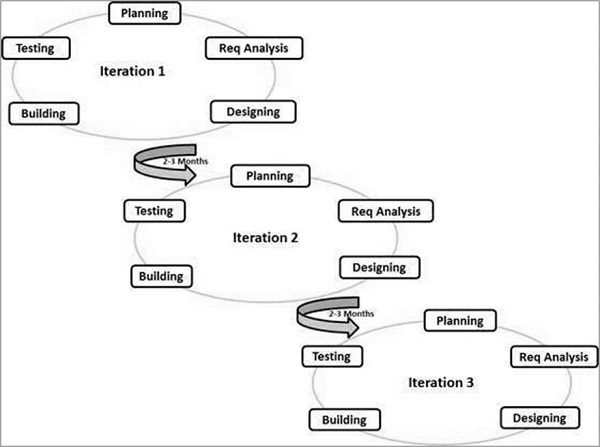
\includegraphics[width=9cm]{agile.jpg}
    \end{center}
    \caption{Agile SDLC model}
    \label{fig:agile}
\end{figure}

The philosophy of Agile is that every project needs to be handled differently and the existing methods
need to be tailored to best suit the project requirements. To deliver specific features for a 
release the tasks are divided into time boxes (small time frames).

Agile uses an iterative approach and  working software build is delivered after each iteration. 
Each build is incremental in terms of features; the final build holds all the features required 
by the customer. Refer to figure \ref{fig:agile}.

Following are the Agile Manifesto principles:

\begin{itemize}
    \item \textbf{Working software:} The best means of communication with the customers to understand
    their requirements is by using demo working software, instead of just depending on documentation.
     
    \item \textbf{Customer collaboration:} Continuous customer interaction is very important to get proper
    requirements, as the requirements cannot be gathered completely in the beginning of the project due 
    to various factors.

    \item \textbf{Responding to change:} The focus is on quick response to changes and 
    continuous development in agile development.
\end{itemize}

\subsection{Agile v/s traditional SDLC Models}

Traditional SDLC models are based on a predictive approach. Teams in traditional SDLC models 
usually work with detailed planning and have a complete view of the exact tasks and features 
to be delivered during the product life cycle. These models entirely depend on the requirement 
analysis and planning done in the beginning of the product life cycle. Any changes to be done go 
through a strict change control management and prioritization.~\cite{agile}

On the other hand Agile uses an adaptive approach where there is no detailed planning and clarity
of what features need to be developed in future. The team adapts to the  changing product requirements 
dynamically. Agile has minimum failure as the product is tested frequently through the release iterations.

The backbone of agile methodology is customer interaction  and open communication with minimum 
documentation are the typical features of agile. The teams in agile methodology are in close collaboration 
with each other and are often based in the same geographical location.

\subsubsection{Pros}

\begin{itemize}
    \item Agile is a very realistic approach to software development.
    \item Functionality can be developed, rapidly demonstrated and promotes teamwork and cross training. 
    \item Resource requirements are minimum.
    \item It delivers early partial working solutions and is suitable for fixed or changing requirements.
    \item Good model for environments that change steadily.
    \item Minimal rules, documentation easily employed and little or no planning required.
    \item Gives flexibility to developers.
\end{itemize}

\subsubsection{Cons}

\begin{itemize}
    \item Not suitable for handling complex dependencies and more risk of sustainability, maintainability and extensibility.
    \item Strict delivery management dictates the scope, functionality to be delivered, and adjustments to meet the deadlines.
    \item Depends heavily on customer interaction, so if the customer is not clear, the team can be driven in the wrong direction.
    \item Has a very high individual dependency, since there is minimum documentation generated and transfer of technology to new 
    team members may be quite challenging due to lack of documentation.
\end{itemize}

\subsection{Why Agile?}

Flexibility and time management are important factors to consider when working on projects.
Working iteratively, as Agile necessitates, allows a project team to deliver operational solutions in incremental builds.
Each incremental change made to the code repository is thus maintained, and product releases are thus ensured to have minimal errors.
Furthermore, tests are also performed prior to every product release, which help find bugs and mitigate errors which 
could have crept into the product during development.

It is also important to note that the JAMstack, which is the technology stack used to implement the project, 
has features which include loose-coupling between modules, and a very wide community of developers. Each module, 
called a microservice, can be easily maintained by individual developers. Since each microservice delivers a limited 
set of functions, documentation for each module can be minimised. JAMstack approaches project development in a 
similar way to Agile, and thus can be a perfect fit.

\section{CI/CD pipeline}

A CI/CD pipeline automates the software delivery process. The pipeline builds codes, runs test (CI),
and safely deploys a new version of the application (CD).

\subsection{CI and CD}

CI stands for Continuous Integration. It is a development process in which the developers merge
their code changes multiple times a day in a central repository. With CI, each change in code 
triggers an automated build and test sequence.

CD stands for Continuous Delivery which on top of continuous integration adds the practice of 
automating the entire software release process. CD includes infrastructure provisioning and deployment 
which may be manual and consists of multiple stages.~\cite{CICD}

\subsection{Elements of CI/CD}

\begin{figure}[h!]
    \begin{center}
        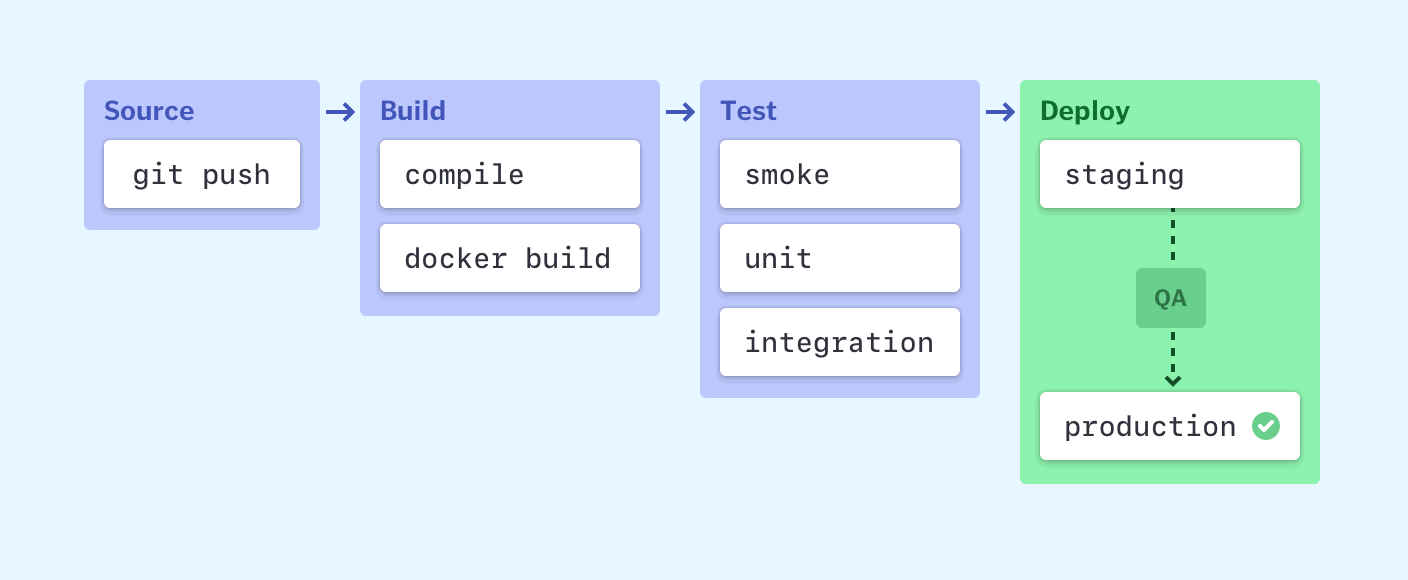
\includegraphics[width=15cm]{cicd.png}
    \end{center}
    \caption{Elements of CI/CD}
    \label{fig:cicd}
\end{figure}

\subsubsection{Source Stage}

Source repository triggers a pipeline run. A notification is triggered to the CI/CD tool 
which runs the corresponding pipeline if there is a change in code. 

\subsubsection{Build Stage}

To build a runnable instance of the product that which can potentially be shipped to end users  
the source code and its dependencies will need to undergo a build stage. 
Programs written in languages such as Java, C/C++, or Go need 
to be compiled, whereas Ruby, Python and JavaScript programs work without this step.

Regardless of the language, cloud-native software is typically deployed with Docker, in which case this 
stage of the CI/CD pipeline builds the Docker containers.

There are fundamental problems in the project's configuration if the project fails to pass the build 
stage, and it’s best to address the problems immediately.

\subsubsection{Test Stage}

Automated tests can be run to validate the code and the behaviour of the product. This stage acts as a safety
net that does not allow the bugs to reach the end-users.

This stage can last from seconds to hours depending on the complexity of the project.

Failure in this stage shows the errors in the code that developers didn't foresee when writing the code.

\subsubsection{Deploy Stage}

Once the runnable instance of the code has passed all the test stages, it is ready to deploy. There are 
multiple deploy environments for example “beta” environment for the product team and “production” 
environment for end-users.

Teams that have embraced the Agile model of development guided by tests and real-time monitoring usually 
deploy work-in-progress manually to a beta environment for additional manual testing and review, and 
automatically deploy approved changes from the master branch to production.

\section{JAMstack}

\subsection{What is JAMstack?}

Jamstack is an architecture designed to make the web faster, more secure, and easier to scale. 
It builds on many of the tools and workflows which bring maximum productivity.

It adheres to the following components : Javascript, APIs and Markup.

The core principles of pre-rendering and decoupling, enable sites and applications to be delivered 
with greater confidence and resilience than ever before.

\subsection{Why use JAMstack?}

These are the core concepts that makes JAMstack deliver fast, secure, high-performing, resilient, and efficient infrastructure:

\subsubsection{Speed}

Serving JAMstack apps as static files directly from a Content Delivery Network makes it 
likely apps will load faster. Therefore the server need not spend time building the page 
before responding; all as a result of pre-rendering. 

\subsubsection{Cost}

More often than not, JAMstack sites are going to run cheaper than their server side counterparts. 
Hosting static assets is cheap and now the pages are being served at the same rate.

\subsubsection{Scalability}

Since the files are being served off of static hosting, likely a CDN, 
that pretty much automatically gives infinite and inexpensive scalability.

\subsubsection{Maintenance}

The static site isn’t hosted on a server, meaning hardware maintenance is offloaded. 
Static HTML, CSS, and JS are maintained headache-free on an automated, distributed CDN system.

\subsubsection{Security}

With JAMstack, there is no need to lockdown all the services as a central organisation, instead, 
each service can be locked in separate containerised services, leading to easier management and isolation.

\subsection{A Comparison with  the Traditional Web Architecture}

Jamstack is the new standard architecture for the web. Using Git workflows and modern build tools, pre-rendered content 
is served to a CDN and made dynamic through APIs and serverless functions. Technologies in the stack include JavaScript frameworks, 
Static Site Generators, Headless CMSs, and CDNs. Refer to figure \ref{fig:jamstack}

\begin{figure}[h!]
    \begin{center}
        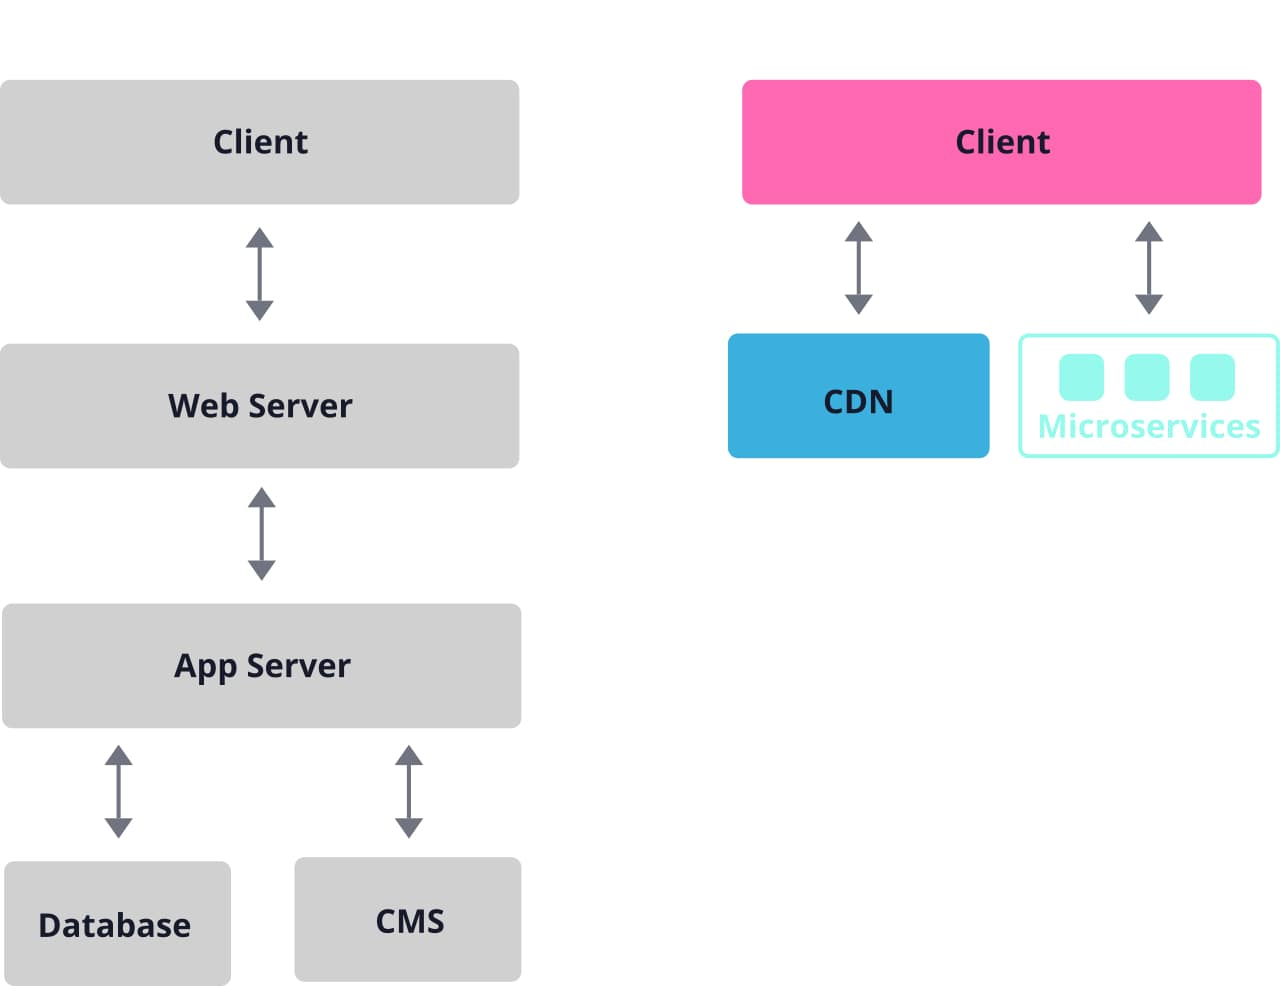
\includegraphics[width=15cm]{Jamstack.jpg}
    \end{center}
    \caption{Traditional web v/s JAMstack}
    \label{fig:jamstack}
\end{figure}

\section{High Level Systems}

\begin{figure}[h]
    \centering
    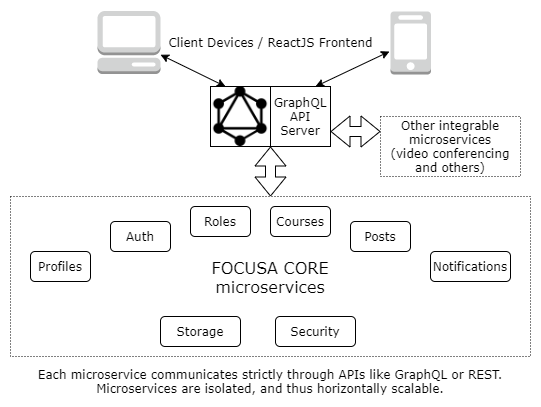
\includegraphics[width=12cm]{highlevel.png}
    \caption{High Level Diagram illustrating all microservices of the project.}
    \label{fig:highlevel}
\end{figure}

Microservices, also known as the microservice architecture, is an architectural style that structures an 
application as a collection of services that are
\begin{itemize}
    \item Highly maintainable and testable
    \item Loosely coupled
    \item Independently deployable
\end{itemize}

The microservice architecture enables the rapid, frequent and reliable delivery of large, complex applications.
The benefits of decomposing an application into different, smaller services are:
\begin{itemize}
    \item \textbf{Modularity:} This makes the application easier to understand, develop, test, and 
    become more resilient to architecture erosion.
    \item \textbf{Scalability:} Since microservices are implemented and deployed independently of 
    each other, i.e. they run within independent processes, they can be monitored and scaled independently.
    \item \textbf{Integration of heterogeneous and legacy systems:} Microservices are considered as a 
    viable mean for modernizing existing monolithic software application.
    \item \textbf{Distributed development:} It parallelizes development by enabling small autonomous teams to
    develop, deploy and scale their respective services independently. It also allows the architecture of 
    an individual service to emerge through continuous refactoring.
\end{itemize}

The project, FOCUSA includes the following microservices. Refer to figure \ref{fig:highlevel}:
\begin{itemize}
    \item \textbf{Auth:} performs the authentication process based on a username and password, and returns refresh cookies with a JWT.
    \item \textbf{Roles:}  returns the roles that a user belongs to. It depicts the different roles that different admins perform.
    \item \textbf{Profiles:} Each user has a unique profile, containing details like the user display picture, username, and the various courses the user has subscribed to.
    \item \textbf{Courses:}  returns the details of the courses which includes the course title and the different users subscribed to the course, as well as a provision for new users to subscribe to the course. Only users with certain roles can moderate their respective courses.
    \item \textbf{Posts:} refers to posts posted by the course moderators. The moderators are able to perform CRUD operations on these posts
    \item \textbf{Notifications:}  pushes notifications to the user devices and also monitors the database for changes.
\end{itemize}

\subsection{Using GraphQL with the Microservices}

The projext will make use of a single GraphQL Schema as an API Gateway to all the microservices, 
integrating it under a single application. This enables easy integration of data from the different services.

One of the main benefits of having everything behind a single endpoint, is that data can be routed more 
effectively than if each request had its own service. 

The microservices handle the business logic themselves, while the GraphQL platform interacts with the 
clients to process the queries by consulting the services using REST API, thus allowing for easier isolation 
and horizontal scaling.

% Activity Diagram
\section{Activity Diagram}

\begin{figure}[h!]
    \begin{center}
        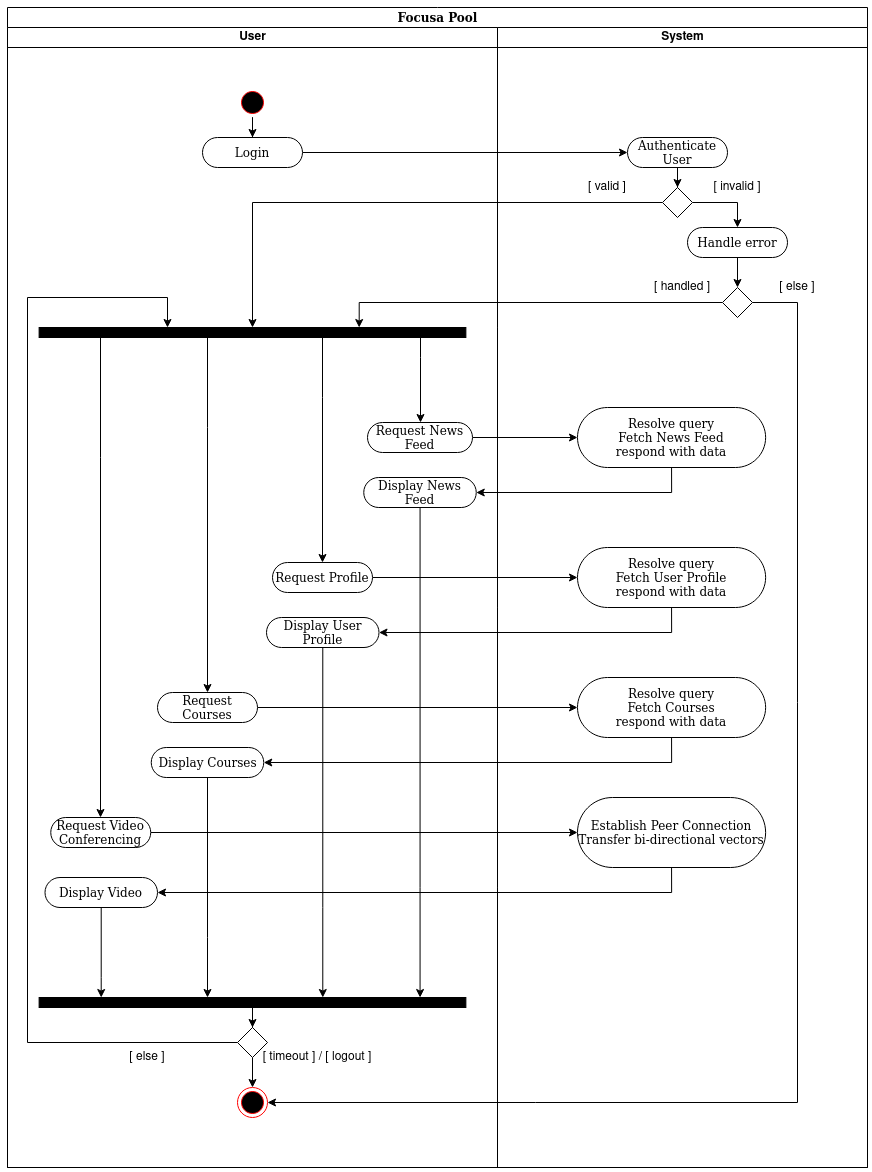
\includegraphics[width=15cm]{activity.png}
    \end{center}
    \caption{Activity Diagram}
    \label{fig:activity}
\end{figure}

Refer to figure \ref{fig:activity}. The user logs in to the app by putting in the valid credentials.
The credentials put in by the user are validated by the system through the authentication mechanism on the server.
If the credentials are found to be incorrect, the system runs the error handler to address the error occurred.
If the user still is not able to produce the correct credentials, the process ends and the user is not allowed to use the app.

If the user has been validated and is found to be genuine, is directed to the home/main page of the app where he can choose to request for the News Feed, User Profile, Courses or launch video conferencing.
All these requests can be made through the navigation panel provided in the app and are accessed as parallel activities.

Once the user requests for a service, the request is sent to the system as a query which is then resolved by the GraphQL to extract the specific requested data from the backend and the response returned is then displayed to the user in structured format.

If the user requests to launch the video conferencing, the system estblishes a peer to peer connection with the requested user system, asks the user to grant access to the camera and audio and starts transfering bi-directional vectors as the secure connection is established.
These bi-directional vectors are worked upon by the algorithm used to reduce the bandwidth usage and the output is displayed in the form of video.

If the user decides to log out of the app, it can be accomplished via the corresponding UI component and as a result all the parallel activities combine to close and the user is logged out of the app safely .
The user is also logged out of the app the session times out.

% Schema diagram.
\section{Database Schema Diagram}

\begin{figure}[h!]
    \centering
    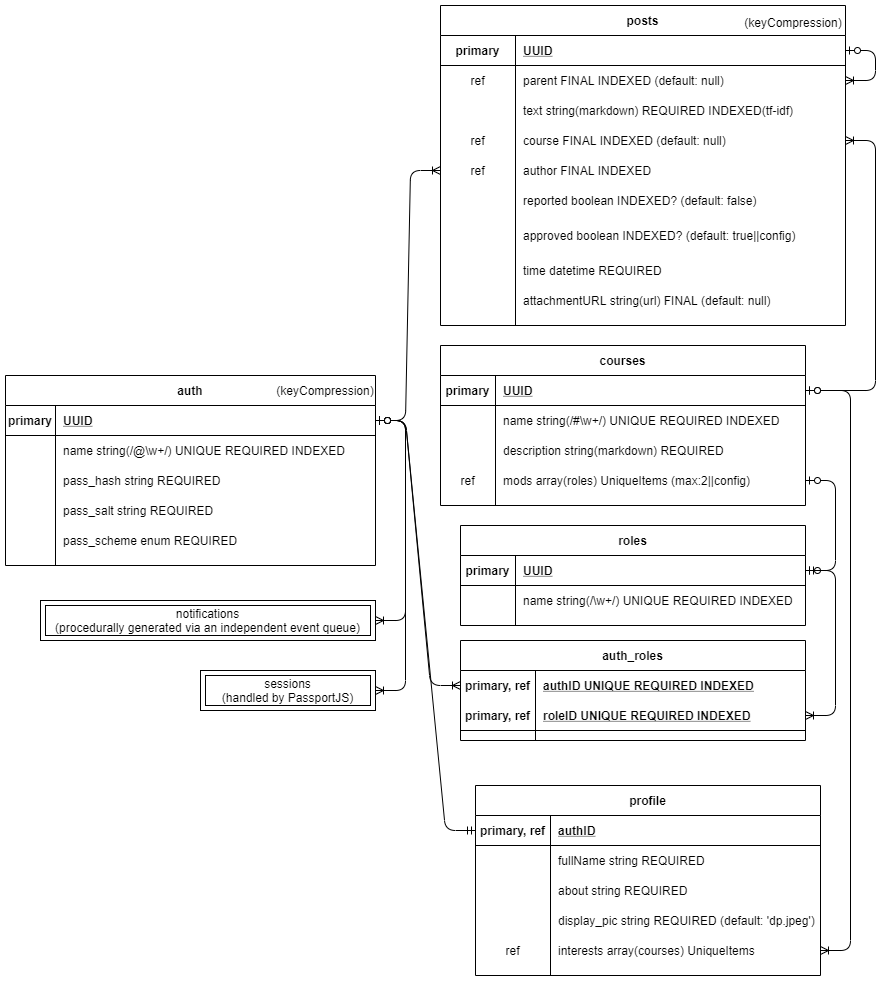
\includegraphics[width=15cm]{db-schema.png}
    \caption{The Database Schema Diagram illustrates the Collections and document schemas, 
    along with relationships between them.}
    \label{fig:schema}
\end{figure}

A database schema represents a \textbf{blueprint} or \textbf{architecture} of how the data will look. 
It describes the shape of the data and how it might relate to other tables or models. Refer to \label{fig:schema}.

The \textbf{Collections} and their respective \textbf{Document Attributes} are:
\begin{enumerate}
    \item \textbf{User}, which describes user details needed for authentication.
    \item \textbf{Posts}, which desribes attributes like text, course, timestamp, URL attachment 
    and flags for reported and approved.
    \item \textbf{Courses}, which includes moderator roles, and describes information which will 
    be displayed to the user, like the course name and description.
    \item \textbf{Roles}, which is collection of roles which any user can have.
    \item \textbf{Profile}, which describes all the extra user details like a full name, display picture, about paragraph, and a list of interests.
\end{enumerate}

The core \textbf{relationships} between the attributes are:
\begin{enumerate}
    \item Each user publishes many posts. One-to-many relationship.
    \item Many users have many roles. Many-to-many relationship.
    \item Each user has a profile. One-to-one relationship with total cardinality.
    \item Many comment posts have one parent post. Many-to-one relationship.
    \item Each post belongs to one course. Many-to-one relationship.
    \item Each course is moderated by many roles. One-to-many relationship.
    \item Each profile subscribes to many courses. One-to-many relationship.
\end{enumerate}

The Posts collection functionally stores all posts and comment documents as simple trees. This data structure can easily support 
and manage a hierarchy similar to tweets in Twitter. However, the moderators will be able to setup a limit to the depth of comments.

\section{Sequence Diagram}

\begin{figure}[h!]
    \begin{center}
        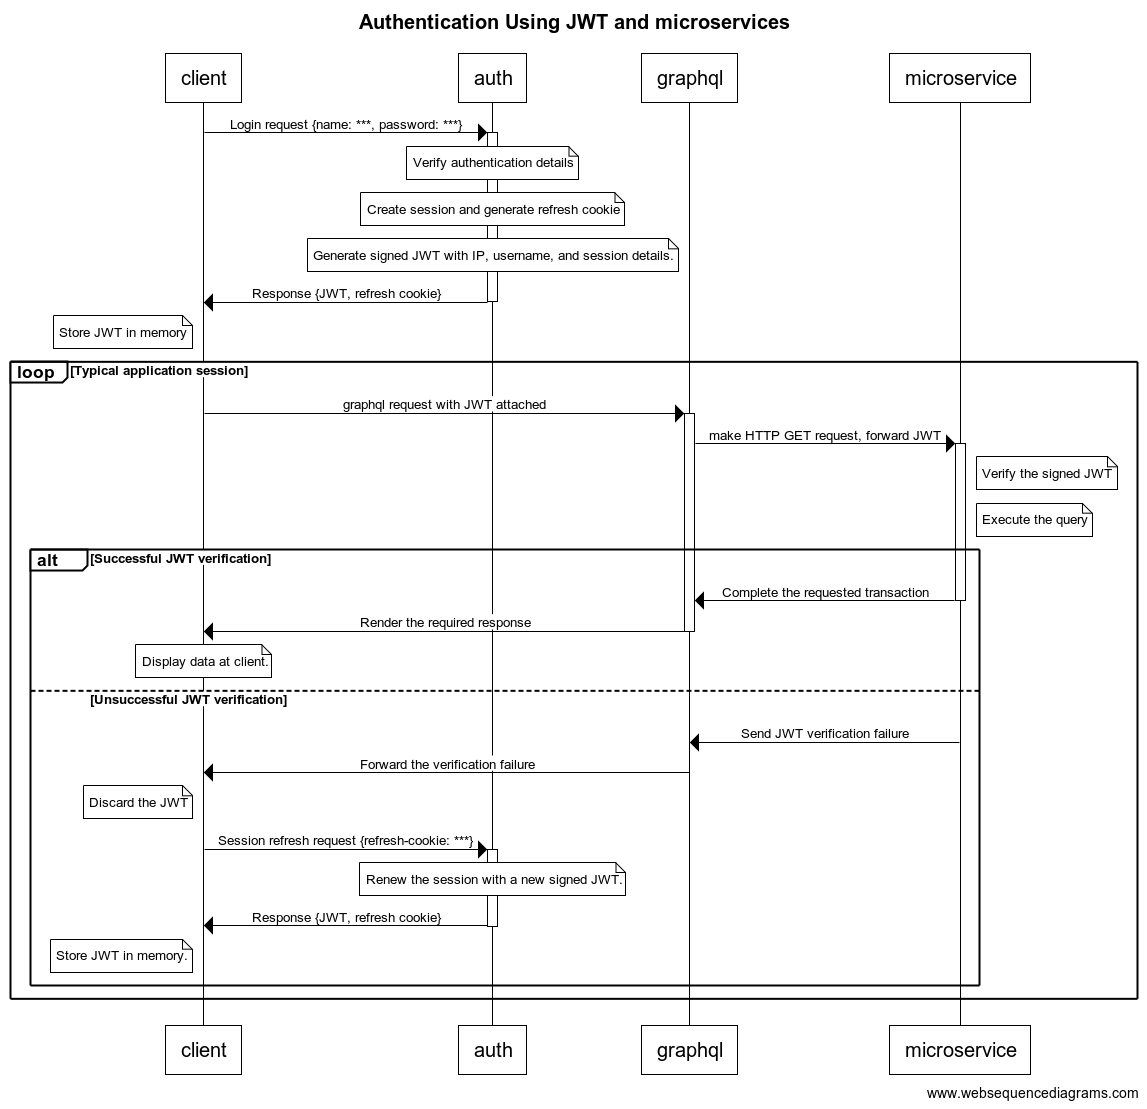
\includegraphics[width=15cm]{sequence.png}
    \end{center}
    \caption{Authentication Sequence Diagram. This diagram illustrates 
    four actors: client, auth, GraphQL, microservice.}
    \label{fig:sequence}
\end{figure}

Refer to figure \ref{fig:sequence}.
The User initiates with a request to login to the Authenticator along with their credentials ie; name and password.
On receiving the credentials, the Authenticator verifies them, creates a session and generates a refresh cookie.
Auth also generates a signed JWT(JSON Web Token) conatining the IP, username and session details of the User.

This JWT is stored in the User's device memory. This JWT is synonymous to an ID card which can be used by 
the User to directly work with the GraphQL and Services without needing to disturb the Authenticator repeatedly.

The User can now communicate with GraphQL by sharing the JWT.
GraphQL makes a request and forwards JWT to the Services. Services here refer to all the microservices that form the system.
The Services validate the signed JWT received from the GraphQL (by checking its digital signature) 
and if found valid execute the query and return response data to GraphQL.
GraphQL then converts the recevied response into the format requested by the User, and sends it to the User.

However, if the Services find the JWT to be invalid, a failure response is sent to
GraphQL which then returns a failure response to the User.
The User now needs to request the Authenticator for a session refresh upon which the Authenticator
returns a new signed JWT along with the refresh cookie.

If the User accidentally refreshes their browser, the JWT will get deleted from memory. 
The User will then request for a session refresh, and a new signed JWT will be generated.

On logout the JWT is simply discarded by deleting the object from memory.

% Neural Network architecture diagram.
